% !TeX program = xelatex
\documentclass[a4paper,10pt]{article}

% ============================================================================
% សន្លឹកកិច្ចការសិស្សបំពេញចន្លោះ ស-ខ្មៅ និងប្លង់ក្ដារខៀន/ចម្លើយគ្រូ (គ្មាន LCD / គ្មានកន្ត្រៃ)
% មេរៀនទី៦ (១-២)៖ កន្សោមសនិទាន និងតម្លៃលេខនៃកន្សោមសនិទាន — ត្រូវគ្នានឹង LS_Plan_RAT61.tex
% ============================================================================
\usepackage[a4paper, left=1.0cm, right=1.0cm, top=0.75cm, bottom=1.00cm, footskip=0.52cm]{geometry}
\usepackage{amsmath}
\usepackage{unicode-math}
\usepackage{fontspec}
\usepackage{array, colortbl}
\usepackage[table]{xcolor}
\usepackage{enumitem}
\usepackage{pifont}
\usepackage{fancyhdr}
\usepackage{lastpage}
\usepackage{tikz}
\usepackage[most]{tcolorbox}
\usetikzlibrary{calc, arrows.meta, decorations.pathreplacing, positioning, babel}

\makeatletter
\let\@expl@@@mark@update@singlecol@structures@@\relax
\makeatother

\providecommand{\NGSFindFonts}{%
  \IfFileExists{C:/Windows/Fonts/cambria.ttc}{%
    \def\NGSSysPath{C:/Windows/Fonts/}%
    \def\NGSUserPath{C:/Users/KIT/AppData/Local/Microsoft/Windows/Fonts/}%
  }{%
    \IfFileExists{./fonts/KhmerOSsiemreap.ttf}{\def\NGSSysPath{./fonts/}\def\NGSUserPath{./fonts/}}{%
    \IfFileExists{../fonts/KhmerOSsiemreap.ttf}{\def\NGSSysPath{../fonts/}\def\NGSUserPath{../fonts/}}{%
    \IfFileExists{../../fonts/KhmerOSsiemreap.ttf}{\def\NGSSysPath{../../fonts/}\def\NGSUserPath{../../fonts/}}{%
    \IfFileExists{../../../fonts/KhmerOSsiemreap.ttf}{\def\NGSSysPath{../../../fonts/}\def\NGSUserPath{../../../fonts/}}{%
    \IfFileExists{../../../../fonts/KhmerOSsiemreap.ttf}{\def\NGSSysPath{../../../../fonts/}\def\NGSUserPath{../../../../fonts/}}{%
    \IfFileExists{../../../../../fonts/KhmerOSsiemreap.ttf}{\def\NGSSysPath{../../../../../fonts/}\def\NGSUserPath{../../../../../fonts/}}{%
    \IfFileExists{../../../../../../fonts/KhmerOSsiemreap.ttf}{\def\NGSSysPath{../../../../../../fonts/}\def\NGSUserPath{../../../../../../fonts/}}{%
      \def\NGSSysPath{../../../../../../../fonts/}\def\NGSUserPath{../../../../../../../fonts/}%
    }}}}}}}%
  }%
}
\NGSFindFonts

\setmathfont[Path={\NGSSysPath}, FontIndex=1, Scale=1.02]{cambria.ttc}
\defaultfontfeatures{Ligatures=TeX}

\setmainfont[
  Path={\NGSUserPath}, Extension=.ttf, Script=Khmer,
  BoldFont={KhmerOSsiemreap}, BoldFeatures={FakeBold=1.8},
  ItalicFont={KhmerOSsiemreap}, ItalicFeatures={FakeSlant=0.25},
  BoldItalicFont={KhmerOSsiemreap}, BoldItalicFeatures={FakeBold=1.8, FakeSlant=0.25}
]{KhmerOSsiemreap}

\newfontfamily\muol[Path={\NGSUserPath}, Extension=.ttf, Script=Khmer]{KhmerOSmuollight}
\newfontfamily\TimesEn[Path={\NGSSysPath}, Extension=.ttf, BoldFont={timesbd}, ItalicFont={timesi}, BoldItalicFont={timesbi}]{times}
\newfontfamily\CalibriFont[Path={\NGSSysPath}, Extension=.ttf]{calibri}

\XeTeXlinebreaklocale "km"
\XeTeXlinebreakskip = 0pt plus 1pt minus 0.1pt

\definecolor{panelgray}{gray}{0.94}
\definecolor{headgray}{gray}{0.85}

\pagestyle{fancy}
\fancyhf{}
\renewcommand{\headrulewidth}{0pt}
\fancyfoot[L]{\fontsize{7.4pt}{9.5pt}\selectfont អនុវិទ្យាល័យព្រះក្រសាំង \en{|} គ្រូ៖ ហុក ប៊ុនថែន \en{|} មេរៀនទី៦ (១--២) សញ្ញាណនិងតម្លៃលេខនៃកន្សោមសនិទាន \en{|} ថ្ងៃចន្ទ ទី១៤ ខែធ្នូ ឆ្នាំ២០២៦}
\fancyfoot[R]{\fontsize{7.8pt}{10pt}\selectfont ទំព័រ \en{\thepage\ / \pageref{LastPage}}}

\setlength{\parindent}{0pt}
\setlength{\parskip}{0pt}
\setlength{\tabcolsep}{4pt}

\newcommand{\en}[1]{{\TimesEn #1}}
\newcommand{\enbf}[1]{{\TimesEn\bfseries #1}}
\newcommand{\unit}[1]{\,\text{\en{#1}}}
\newcommand{\riel}{\,\text{៛}}
\newcommand{\cnum}[1]{\mbox{\fontsize{10pt}{12pt}\selectfont\ding{\numexpr181+#1\relax}}}
\newcommand{\chkbox}{\tikz[baseline=-0.15ex]\draw[black, line width=0.85pt, fill=white] (0,0) rectangle (0.24cm,0.24cm);}
\newcommand{\ansbox}[1][2.0cm]{\,\tikz[baseline=-0.65ex]\draw[black, line width=0.65pt, fill=white] (0,0) rectangle (#1, 0.42cm);\,}
\newcommand{\dotline}[1][2.2cm]{\makebox[#1]{\dotfill}}

\newcommand{\pagebanner}[2]{%
  \begin{tcolorbox}[
    enhanced, sharp corners, colback=headgray, colframe=black,
    boxrule=1.05pt, boxsep=1pt, top=2.5pt, bottom=2.5pt, left=6pt, right=6pt,
    after skip=3.5pt
  ]
    {\muol\fontsize{9.0pt}{13.2pt}\selectfont #1}\hfill{\fontsize{8.0pt}{11.2pt}\selectfont\textbf{#2}}
  \end{tcolorbox}%
}

\newcommand{\secstrip}[2]{%
  \vspace{3pt}%
  \begin{tcolorbox}[
    enhanced, sharp corners, colback=panelgray, colframe=black,
    boxrule=0.8pt, boxsep=0.8pt, top=2pt, bottom=2pt, left=5pt, right=5pt,
    after skip=3pt
  ]
    {\muol\fontsize{8.5pt}{12.2pt}\selectfont #1}\hfill{\fontsize{7.8pt}{10.8pt}\selectfont\textit{#2}}
  \end{tcolorbox}%
}

\newcolumntype{L}[1]{>{\raggedright\arraybackslash}p{#1}}
\newcolumntype{C}[1]{>{\centering\arraybackslash}p{#1}}

\begin{document}
\fontsize{9.5pt}{14.5pt}\selectfont

% ============================================================================
% ទំព័រទី ១៖ សន្លឹកកិច្ចការសិស្ស (ផ្នែកមុខ៖ E1 -> E2 -> E3)
% ============================================================================
\pagebanner{សន្លឹកកិច្ចការសិស្ស \enbf{(}៦\enbf{.}១\enbf{--}៦\enbf{.}២ សញ្ញាណនិងតម្លៃលេខនៃកន្សោមសនិទាន\enbf{)} \enbf{--} ផ្នែកមុខ}{ថ្នាក់ទី៨ \en{|} ទំ.៧៥--៧៦}

\begin{tcolorbox}[
  enhanced, sharp corners, colback=white, colframe=black,
  boxrule=0.8pt, boxsep=1.5pt, top=3.5pt, bottom=3.5pt, left=5pt, right=5pt,
  after skip=4pt
]
  \fontsize{9.0pt}{13.0pt}\selectfont
  \textbf{ឈ្មោះសិស្ស៖} \dotline[4.3cm] \quad
  \textbf{សមាជិកក្រុម៖} \dotline[4.3cm] \quad
  \textbf{ថ្នាក់ទី៖} ៨\dotline[0.9cm] \quad
  \textbf{ក្រុមទី៖} \dotline[1.0cm]
\end{tcolorbox}

% --- E1 Engage ---
\secstrip{ផ្នែកទី ១ \enbf{(E1 - Engage)} ៖ បេសកកម្មវិនិច្ឆ័យ «ស្មើសូន្យ» ឬ «គ្មានន័យ»}{រយៈពេល ៣ នាទី (គូស \ding{51} ក្នុង \chkbox)}

\begin{tcolorbox}[
  enhanced, sharp corners, colback=white, colframe=black,
  boxrule=0.8pt, boxsep=2.5pt, top=4pt, bottom=4pt, left=6pt, right=6pt
]
  គេឱ្យកន្សោមសនិទាន $\dfrac{a - 5}{2a + 6}$ (ទំ.៧៦) ។ តើការអះអាងរបស់សិស្សរូបណាត្រឹមត្រូវ?\\[3pt]
  \chkbox\ \textbf{សិស្ស ក៖} ចំពោះ $a = -3$ ភាគបែងស្មើ $0$ ដូចនេះកន្សោមស្មើសូន្យ \quad
  \chkbox\ \textbf{សិស្ស ខ៖} $a = -3$ គ្មានន័យ ឯ $a = 5$ ទើបស្មើសូន្យ\\[3pt]
  $\bullet$ \textbf{សាកល្បងជំនួស៖} ពេល $a = -3$ បាន $\dfrac{-3-5}{2(-3)+6} =$ \ansbox[1.8cm]; \quad ពេល $a = 5$ បាន $\dfrac{5-5}{2(5)+6} =$ \ansbox[1.8cm] ។
\end{tcolorbox}

\vspace{3pt}

% --- E2 Explore ---
\secstrip{ផ្នែកទី ២ \enbf{(E2 - Explore)} ៖ ស្គាល់កន្សោមសនិទាន និងគណនាតម្លៃលេខ (ទំ.៧៥--៧៦)}{រយៈពេល ១១ នាទី}

\textbf{សកម្មភាព ១ (\en{E2-A} — ៥ នាទី)៖ ចាត់ថ្នាក់កន្សោមសនិទាន និងមិនមែនសនិទាន (ទំ.៧៥)}

\begin{tcolorbox}[
  enhanced, sharp corners, colback=white, colframe=black,
  boxrule=0.8pt, boxsep=2.5pt, top=4pt, bottom=4pt, left=6pt, right=6pt
]
  គូស \ding{51} មុខកន្សោមសនិទាន និងគូស \ding{55} មុខកន្សោមដែល\textbf{មិនមែន}ជាកន្សោមសនិទាន៖\\[3pt]
  \chkbox\ ក) $\dfrac{x}{y}$ \qquad\quad
  \chkbox\ ខ) $\dfrac{a + b}{b}$ \qquad\quad
  \chkbox\ គ) $\dfrac{1 + x}{x^2 - 1}$ \qquad\quad
  \chkbox\ ឃ) $\dfrac{x}{\sqrt{y}}$\\[3pt]
  $\bullet$ \textbf{សង្កេត៖} កន្សោម $\dfrac{x}{\sqrt{y}}$ ពុំមែនជាកន្សោមសនិទានទេ ព្រោះភាគបែង $\sqrt{y}$ ពុំមែនជា \dotline[3.8cm] ។
\end{tcolorbox}

\vspace{4pt}
\textbf{សកម្មភាព ២ (\en{E2-B} — ៦ នាទី)៖ គណនាតម្លៃលេខនៃកន្សោម $\dfrac{3x}{x - 2}$ (ទំ.៧៦ ឧទាហរណ៍)}

\begin{tcolorbox}[
  enhanced, sharp corners, colback=white, colframe=black,
  boxrule=0.8pt, boxsep=2.5pt, top=4pt, bottom=4pt, left=6pt, right=6pt
]
  $\bullet$ \textbf{១) ចំពោះ $x = -1$៖} $\dfrac{3(-1)}{-1 - 2} = \dfrac{-3}{-3} =$ \ansbox[1.8cm] \qquad
  \textbf{២) ចំពោះ $x = 0$៖} $\dfrac{3 \times 0}{0 - 2} = \dfrac{0}{-2} =$ \ansbox[1.8cm]\\[4pt]
  $\bullet$ \textbf{៣) ចំពោះ $x = 2$៖} ភាគបែង $x - 2 = 2 - 2 =$ \ansbox[1.5cm] ក្នុងករណីនេះ កន្សោម \dotline[3.4cm] !
\end{tcolorbox}

\vfill

% --- E3 Explain ---
\secstrip{ផ្នែកទី ៣ \enbf{(E3 - Explain)} ៖ សង្ខេបនិយមន័យ លក្ខខណ្ឌទាំង ៣ និងធនាគារហេតុផល \enbf{B\&W}}{រយៈពេល ៦ នាទី}

\begin{tcolorbox}[
  enhanced, sharp corners, colback=white, colframe=black,
  boxrule=0.85pt, boxsep=2.5pt, top=4pt, bottom=4pt, left=6pt, right=6pt
]
  $\bullet$ \textbf{១) និយមន័យ៖} កន្សោមសនិទានជាកន្សោមមានទម្រង់ \ansbox[1.8cm] ដែល $A$ និង $B$ ជាឯកធា ឬពហុធា ($B \neq 0$)\\[4pt]
  $\bullet$ \textbf{២) លក្ខខណ្ឌមានន័យ និងគ្មានន័យ៖} មានន័យលុះត្រាតែភាគបែង \ansbox[2.0cm]; \quad គ្មានន័យកាលណាភាគបែង \ansbox[2.0cm]\\[4pt]
  $\bullet$ \textbf{៣) លក្ខខណ្ឌស្មើនឹងសូន្យ៖} $\dfrac{A}{B} = 0$ លុះត្រាតែភាគយក \ansbox[2.2cm] និងភាគបែង \ansbox[2.2cm]\\[4pt]
  \tikz\draw[black, dashed, line width=0.6pt] (0,0) -- (\linewidth,0);\\[3pt]
  \fontsize{8.8pt}{13.0pt}\selectfont
  \textbf{ធនាគារហេតុផល (\en{Warrant Bank})៖} \quad
  \cnum{1} $A, B$ ជាឯកធា/ពហុធា (គ្មាន $\sqrt{y}$) \quad
  \cnum{2} មានន័យ $\iff B \neq 0$\\
  \cnum{3} គ្មានន័យ $\iff B = 0$ (ចែកនឹងសូន្យមិនបាន) \quad
  \cnum{4} ស្មើសូន្យ $\iff A = 0$ និង $B \neq 0$
\end{tcolorbox}

% ============================================================================
% ទំព័រទី ២៖ សន្លឹកកិច្ចការសិស្ស (ផ្នែកខាងខ្នង៖ E4 -> E5 -> កិច្ចការផ្ទះ)
% ============================================================================
\clearpage
\pagebanner{សន្លឹកកិច្ចការសិស្ស \enbf{(}៦\enbf{.}១\enbf{--}៦\enbf{.}២ សញ្ញាណនិងតម្លៃលេខនៃកន្សោមសនិទាន\enbf{)} \enbf{--} ផ្នែកខ្នង}{ថ្នាក់ទី៨ \en{|} ទំ.៧៥--៧៦, ៨៥}

% --- E4 Elaborate ---
\secstrip{ផ្នែកទី ៤ \enbf{(E4 - Elaborate)} ៖ លំហាត់គំរូ និងប្រតិបត្តិពង្រីក (ទំ.៧៥--៧៦)}{រយៈពេល ១០ នាទី}

\begin{tcolorbox}[
  enhanced, sharp corners, colback=white, colframe=black,
  boxrule=0.8pt, boxsep=2.5pt, top=4pt, bottom=4pt, left=6pt, right=6pt
]
  \textbf{១) លំហាត់គំរូ (ទំ.៧៥) — សរសេរជាកន្សោមសនិទាន៖}\\[3pt]
  \hspace*{0.3cm}$\bullet$ ក) ផលធៀបនៃពីរចំនួនគត់តគ្នា $n$ និង $n+1$៖ \ansbox[2.4cm] \quad
  ខ) ផ្ទៃធៀបបរិមាត្រចតុកោណកែងវិមាត្រ $x, y$៖ \ansbox[2.8cm]\\[4pt]
  \textbf{២) លំហាត់គំរូ (ទំ.៧៦) — កន្សោមសនិទាន $\dfrac{a - 5}{2a + 6}$៖}\\[3pt]
  \hspace*{0.3cm}$\bullet$ ក) គ្មានន័យពេល $2a + 6 = 0 \implies a =$ \ansbox[2.0cm] \qquad
  ខ) ស្មើសូន្យពេល $a - 5 = 0 \implies a =$ \ansbox[2.0cm]\\[4pt]
  \textbf{៣) ប្រតិបត្តិ (ទំ.៧៦) — កន្សោមសនិទាន $\dfrac{4}{x^2 + 1}$៖} ចំពោះ $x = -1$ បាន \ansbox[1.6cm]; \ ចំពោះ $x = 1$ បាន \ansbox[1.6cm]\\[3pt]
  \textbf{ឆ្លុះបញ្ចាំង (\en{EIA Looking-Back})៖} ហេតុអ្វី $\dfrac{4}{x^2 + 1}$ មានន័យគ្រប់ $x \in \mathbb{R}$ និងមិនអាចស្មើសូន្យ? \dotline[4.2cm] ។
\end{tcolorbox}

\vspace{4pt}

% --- E5 Evaluate ---
\secstrip{ផ្នែកទី ៥ \enbf{(E5 - Evaluate)} ៖ ប្រតិបត្តិ (ទំ.៧៥, ៨៥) សំណួរវិនិច្ឆ័យ \enbf{A--D} និងសំបុត្រចេញ}{រយៈពេល ១០ នាទី}

\begin{tcolorbox}[
  enhanced, sharp corners, colback=white, colframe=black,
  boxrule=0.8pt, boxsep=2.5pt, top=4pt, bottom=4pt, left=6pt, right=6pt
]
  \textbf{១) ប្រតិបត្តិជាក្រុម (ទំ.៧៥ និង ទំ.៨៥ \en{\#2, \#3, \#4})៖}\\[3pt]
  \hspace*{0.3cm}$\bullet$ ប្រតិបត្តិ ទំ.៧៥ (ផ្ទៃរង្វង់កាំ $r$ ធៀបការេជ្រុង $x$)៖ \ansbox[2.4cm] \quad
  \en{\#2} ក ($\dfrac{7x}{6x+7}$ មានន័យ)៖ \ansbox[2.8cm]\\[3pt]
  \hspace*{0.3cm}$\bullet$ \en{\#2} គ ($\dfrac{x+1}{(x+4)(x-3)}$ មានន័យ)៖ \ansbox[2.2cm] \
  \en{\#3} ក ($\dfrac{a}{a-1}$ គ្មានន័យ)៖ \ansbox[1.4cm] \
  \en{\#4} ក ($\dfrac{2x-3}{2x} = 0$)៖ \ansbox[1.4cm]\\[4pt]
  \textbf{២) បិទបេសកកម្ម \en{E1}៖} សិស្ស \dotline[1.1cm] ត្រឹមត្រូវ ព្រោះ $a = -3$ ធ្វើឱ្យកន្សោម \dotline[2.4cm] ឯ $a = 5$ ទើបស្មើ $0$ ។
\end{tcolorbox}

\vspace{4pt}

\begin{tcolorbox}[
  enhanced, sharp corners, colback=white, colframe=black,
  boxrule=0.85pt, boxsep=2.5pt, top=4pt, bottom=4pt, left=6pt, right=6pt
]
  \textbf{៣) សំណួរវិនិច្ឆ័យ \en{A--D} (តើតម្លៃ $x$ ណាដែលធ្វើឱ្យ $\dfrac{x - 4}{x + 2}$ គ្មានន័យ? — គូសរង្វង់ រួចលើកម្រាមដៃ ១--៤)៖}\\[3pt]
  \textbf{\en{A.}} $x = 4$ \qquad\qquad\quad
  \textbf{\en{B.}} $x = -2$ \qquad\qquad\quad
  \textbf{\en{C.}} $x = 2$ \qquad\qquad\quad
  \textbf{\en{D.}} $x = 0$\\[4pt]
  \tikz\draw[black, dashed, line width=0.6pt] (0,0) -- (\linewidth,0);\\[3pt]
  \textbf{៤) សំបុត្រចេញ ៦០ វិនាទី (ទំ.៨៥ \en{\#2} ខ)៖} កន្សោម $\dfrac{3x}{(x - 3)^2}$ មានន័យលុះត្រាតែ $x$ \ansbox[3.2cm] ។
\end{tcolorbox}

\vfill

% --- Homework Box ---
\begin{tcolorbox}[
  enhanced, sharp corners, colback=panelgray, colframe=black,
  boxrule=0.9pt, boxsep=2.5pt, top=4pt, bottom=4pt, left=6pt, right=6pt
]
  {\muol\fontsize{8.8pt}{13pt}\selectfont កិច្ចការផ្ទះ \enbf{(}សៀវភៅគោល ទំ\enbf{.}៨៥ លេខ ១\enbf{,} ២\enbf{,} ៣\enbf{,} ៤\enbf{)}}\\[3pt]
  $\bullet$ \textbf{១) ទំ.៨៥ \en{\#1} ខ៖} គណនាតម្លៃលេខនៃ $\dfrac{-a^2 + 4}{2a^2 - a - 1}$ ចំពោះ $a = -2$, $a = -\dfrac{1}{2}$ និង $a = 1$ ។\\[2pt]
  $\bullet$ \textbf{២) ទំ.៨៥ \en{\#2} ឃ, \en{\#3} គ, \en{\#4} គ៖} រកតម្លៃអថេរឱ្យ $\dfrac{x^2+12x+32}{x^2-16}$ មានន័យ, $\dfrac{a^2-4a}{(a-1)^2-1}$ គ្មានន័យ និង $\dfrac{(x-5)(2x-1)-x+5}{x^2-4} = 0$ ។
\end{tcolorbox}

% ============================================================================
% ទំព័រទី ៣៖ ទំព័រគ្រូបង្រៀន — ប្លង់ក្ដារខៀន ៣ ផ្នែក (គ្មាន LCD) និងចម្លើយផ្ទៀងផ្ទាត់រហ័ស
% ============================================================================
\clearpage
\pagebanner{ទំព័រគ្រូបង្រៀន ៖ ប្លង់ក្ដារខៀន \enbf{(}គ្មាន \enbf{LCD)} និងចម្លើយផ្ទៀងផ្ទាត់រហ័ស}{៦.១--៦.២ កន្សោមសនិទាន និងតម្លៃលេខ (\en{RAT61})}

\secstrip{១. គំរូប្លង់បែងចែកក្ដារខៀន ៣ ផ្នែក សម្រាប់ថ្នាក់រៀនគ្មាន \enbf{LCD}}{សម្រាប់គ្រូប្រើដីស/ហ្វឺត}

\begin{center}
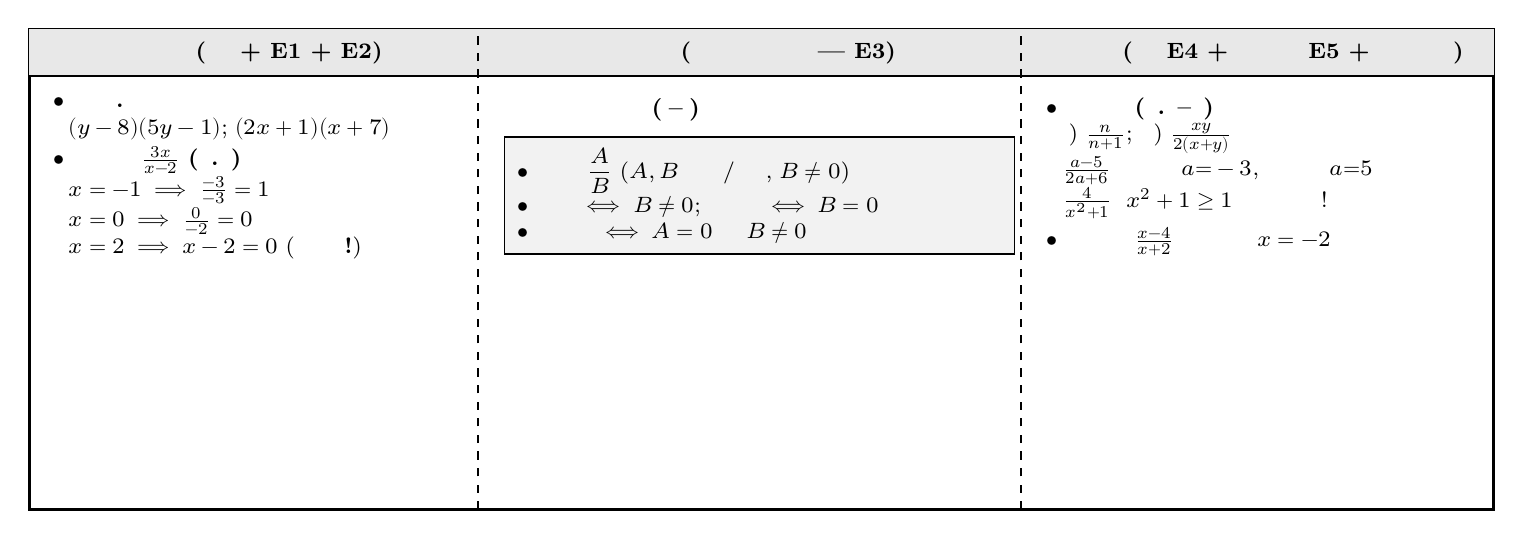
\begin{tikzpicture}[x=1cm, y=1cm, every node/.style={font=\footnotesize, text=black}]
  \draw[black, line width=1.1pt] (0,0) rectangle (18.6,6.1);
  \fill[gray!18] (0,5.50) rectangle (18.6,6.1);
  \draw[black, line width=0.7pt] (0,5.50) -- (18.6,5.50);
  \draw[black, dashed, line width=0.75pt] (5.7,0) -- (5.7,6.1);
  \draw[black, dashed, line width=0.75pt] (12.6,0) -- (12.6,6.1);

  \node at (2.85,5.80) {\textbf{ផ្នែកឆ្វេង (កំណែ + \en{E1} + \en{E2})}};
  \node at (9.15,5.80) {\textbf{ផ្នែកកណ្ដាល (ខ្លឹមសារគោលរក្សាទុក — \en{E3})}};
  \node at (15.60,5.80) {\textbf{ផ្នែកស្ដាំ (គំរូ \en{E4} + ប្រតិបត្តិ \en{E5} + កិច្ចការផ្ទះ)}};

  % Left zone
  \node[anchor=north west, text width=5.3cm] at (0.18,5.35) {
    $\bullet$ \textbf{កំណែ ទំ.៧៤៖}\\
    \hspace*{0.2cm}$(y-8)(5y-1)$; $(2x+1)(x+7)$\\[2pt]
    $\bullet$ \textbf{តម្លៃលេខនៃ $\tfrac{3x}{x-2}$ (ទំ.៧៦)៖}\\
    \hspace*{0.2cm}$x = -1 \implies \tfrac{-3}{-3} = 1$\\
    \hspace*{0.2cm}$x = 0 \implies \tfrac{0}{-2} = 0$\\
    \hspace*{0.2cm}$x = 2 \implies x - 2 = 0$ (\textbf{គ្មានន័យ!})
  };

  % Center zone
  \node[anchor=north west, text width=6.5cm] at (5.90,5.35) {
    {\muol\fontsize{8.2pt}{12pt}\selectfont មេរៀនទី៦៖ កន្សោមសនិទាន \enbf{(}១\enbf{--}២\enbf{)}}\\[3pt]
    \begin{tcolorbox}[enhanced, sharp corners, colback=gray!10, colframe=black, boxrule=0.6pt, boxsep=1.5pt, left=3pt, right=3pt, top=2pt, bottom=2pt]
      $\bullet$ \textbf{ទម្រង់៖} $\dfrac{A}{B}$ ($A, B$ ជាឯកធា/ពហុធា, $B \neq 0$)\\
      $\bullet$ \textbf{មានន័យ} $\iff B \neq 0$; \textbf{គ្មានន័យ} $\iff B = 0$\\
      $\bullet$ \textbf{ស្មើសូន្យ} $\iff A = 0$ និង $B \neq 0$
    \end{tcolorbox}
  };

  % Right zone
  \node[anchor=north west, text width=5.6cm] at (12.80,5.35) {
    $\bullet$ \textbf{លំហាត់គំរូ (ទំ.៧៥--៧៦)៖}\\
    \hspace*{0.2cm}ក) $\tfrac{n}{n+1}$; \ ខ) $\tfrac{xy}{2(x+y)}$\\
    \hspace*{0.2cm}$\tfrac{a-5}{2a+6}$៖ គ្មានន័យ $a{=}-3$, ស្មើសូន្យ $a{=}5$\\
    \hspace*{0.2cm}$\tfrac{4}{x^2+1}$៖ $x^2+1 \ge 1$ មានន័យជានិច្ច!\\[2pt]
    $\bullet$ \textbf{វិនិច្ឆ័យ៖} $\tfrac{x-4}{x+2}$ គ្មានន័យពេល $x = -2$
  };
\end{tikzpicture}
\end{center}

\secstrip{២. ចម្លើយផ្ទៀងផ្ទាត់រហ័សសម្រាប់សន្លឹកកិច្ចការសិស្ស \enbf{(}ទំព័រ ១ និង ទំព័រ ២\enbf{)}}{\en{Answer Key}}

\begin{tcolorbox}[
  enhanced, sharp corners, colback=white, colframe=black,
  boxrule=0.8pt, boxsep=2.5pt, top=4pt, bottom=4pt, left=6pt, right=6pt
]
  $\bullet$ \textbf{ផ្នែក \en{E1}៖} សិស្ស ខ ត្រឹមត្រូវ ($a = -3 \implies \tfrac{-8}{0}$ គ្មានន័យ; $a = 5 \implies \tfrac{0}{16} = 0$) ។\\[2pt]
  $\bullet$ \textbf{ផ្នែក \en{E2}៖} សកម្មភាព ១៖ ក, ខ, គ (\ding{51}), ឃ (\ding{55} មិនមែនឯកធាឬពហុធា) ។ សកម្មភាព ២៖ $1$; $0$; $0$ (កន្សោមគ្មានន័យ) ។\\[2pt]
  $\bullet$ \textbf{ផ្នែក \en{E4}៖} ១) $\tfrac{n}{n+1}$; $\tfrac{xy}{2(x+y)}$; ២) $a = -3$; $a = 5$; ៣) $2$; $2$ ($x^2+1 \ge 1 > 0$ និងភាគយក $4 \neq 0$) ។\\[2pt]
  $\bullet$ \textbf{ផ្នែក \en{E5}៖} ១) $\tfrac{\pi r^2}{x^2}$; $x \neq -\tfrac{7}{6}$; $x \neq -4, 3$; $a = 1$; $x = \tfrac{3}{2}$; ២) សិស្ស ខ; ៣) \textbf{ជម្រើស \en{B}} ($x = -2$); ៤) $x \neq 3$ ។
\end{tcolorbox}

\secstrip{៣. ចម្លើយលម្អិតនៃកិច្ចការផ្ទះ \enbf{(}សម្រាប់គ្រូផ្ទៀងផ្ទាត់នៅដើមម៉ោងបន្ទាប់\enbf{)}}{សៀវភៅគោល ទំ.៨៥}

\begin{tcolorbox}[
  enhanced, sharp corners, colback=white, colframe=black,
  boxrule=0.8pt, boxsep=2.5pt, top=4pt, bottom=4pt, left=6pt, right=6pt
]
  $\bullet$ \textbf{១) ទំ.៨៥ \en{\#1} ខ៖} ចំពោះ $a = -2$ បាន $\dfrac{-4+4}{8+2-1} = \mathbf{0}$; \ ចំពោះ $a = -\dfrac{1}{2}$ បាន $\dfrac{-\frac{1}{4}+4}{\frac{1}{2}+\frac{1}{2}-1} = \dfrac{\frac{15}{4}}{0}$ (\textbf{គ្មានន័យ}); \ ចំពោះ $a = 1$ បាន $\dfrac{3}{0}$ (\textbf{គ្មានន័យ}) ។\\[2pt]
  $\bullet$ \textbf{២) ទំ.៨៥ \en{\#2} ឃ, \en{\#3} គ, \en{\#4} គ៖} \en{\#2} ឃ) $x^2-16 \neq 0 \iff \mathbf{x \neq \pm 4}$; \ \en{\#3} គ) $(a-1)^2-1 = a(a-2) = 0 \iff \mathbf{a = 0,\ 2}$; \ \en{\#4} គ) $2(x-5)(x-1)=0$ និង $x\neq \pm 2 \implies \mathbf{x = 1,\ 5}$ ។
\end{tcolorbox}

\end{document}
